% Options for packages loaded elsewhere
\PassOptionsToPackage{unicode}{hyperref}
\PassOptionsToPackage{hyphens}{url}
\PassOptionsToPackage{dvipsnames,svgnames,x11names}{xcolor}
%
\documentclass[
  letterpaper,
  DIV=11,
  numbers=noendperiod]{scrartcl}

\usepackage{amsmath,amssymb}
\usepackage{iftex}
\ifPDFTeX
  \usepackage[T1]{fontenc}
  \usepackage[utf8]{inputenc}
  \usepackage{textcomp} % provide euro and other symbols
\else % if luatex or xetex
  \usepackage{unicode-math}
  \defaultfontfeatures{Scale=MatchLowercase}
  \defaultfontfeatures[\rmfamily]{Ligatures=TeX,Scale=1}
\fi
\usepackage{lmodern}
\ifPDFTeX\else  
    % xetex/luatex font selection
\fi
% Use upquote if available, for straight quotes in verbatim environments
\IfFileExists{upquote.sty}{\usepackage{upquote}}{}
\IfFileExists{microtype.sty}{% use microtype if available
  \usepackage[]{microtype}
  \UseMicrotypeSet[protrusion]{basicmath} % disable protrusion for tt fonts
}{}
\makeatletter
\@ifundefined{KOMAClassName}{% if non-KOMA class
  \IfFileExists{parskip.sty}{%
    \usepackage{parskip}
  }{% else
    \setlength{\parindent}{0pt}
    \setlength{\parskip}{6pt plus 2pt minus 1pt}}
}{% if KOMA class
  \KOMAoptions{parskip=half}}
\makeatother
\usepackage{xcolor}
\setlength{\emergencystretch}{3em} % prevent overfull lines
\setcounter{secnumdepth}{-\maxdimen} % remove section numbering
% Make \paragraph and \subparagraph free-standing
\ifx\paragraph\undefined\else
  \let\oldparagraph\paragraph
  \renewcommand{\paragraph}[1]{\oldparagraph{#1}\mbox{}}
\fi
\ifx\subparagraph\undefined\else
  \let\oldsubparagraph\subparagraph
  \renewcommand{\subparagraph}[1]{\oldsubparagraph{#1}\mbox{}}
\fi


\providecommand{\tightlist}{%
  \setlength{\itemsep}{0pt}\setlength{\parskip}{0pt}}\usepackage{longtable,booktabs,array}
\usepackage{calc} % for calculating minipage widths
% Correct order of tables after \paragraph or \subparagraph
\usepackage{etoolbox}
\makeatletter
\patchcmd\longtable{\par}{\if@noskipsec\mbox{}\fi\par}{}{}
\makeatother
% Allow footnotes in longtable head/foot
\IfFileExists{footnotehyper.sty}{\usepackage{footnotehyper}}{\usepackage{footnote}}
\makesavenoteenv{longtable}
\usepackage{graphicx}
\makeatletter
\def\maxwidth{\ifdim\Gin@nat@width>\linewidth\linewidth\else\Gin@nat@width\fi}
\def\maxheight{\ifdim\Gin@nat@height>\textheight\textheight\else\Gin@nat@height\fi}
\makeatother
% Scale images if necessary, so that they will not overflow the page
% margins by default, and it is still possible to overwrite the defaults
% using explicit options in \includegraphics[width, height, ...]{}
\setkeys{Gin}{width=\maxwidth,height=\maxheight,keepaspectratio}
% Set default figure placement to htbp
\makeatletter
\def\fps@figure{htbp}
\makeatother

\KOMAoption{captions}{tableheading}
\makeatletter
\makeatother
\makeatletter
\makeatother
\makeatletter
\@ifpackageloaded{caption}{}{\usepackage{caption}}
\AtBeginDocument{%
\ifdefined\contentsname
  \renewcommand*\contentsname{Table of contents}
\else
  \newcommand\contentsname{Table of contents}
\fi
\ifdefined\listfigurename
  \renewcommand*\listfigurename{List of Figures}
\else
  \newcommand\listfigurename{List of Figures}
\fi
\ifdefined\listtablename
  \renewcommand*\listtablename{List of Tables}
\else
  \newcommand\listtablename{List of Tables}
\fi
\ifdefined\figurename
  \renewcommand*\figurename{Figure}
\else
  \newcommand\figurename{Figure}
\fi
\ifdefined\tablename
  \renewcommand*\tablename{Table}
\else
  \newcommand\tablename{Table}
\fi
}
\@ifpackageloaded{float}{}{\usepackage{float}}
\floatstyle{ruled}
\@ifundefined{c@chapter}{\newfloat{codelisting}{h}{lop}}{\newfloat{codelisting}{h}{lop}[chapter]}
\floatname{codelisting}{Listing}
\newcommand*\listoflistings{\listof{codelisting}{List of Listings}}
\makeatother
\makeatletter
\@ifpackageloaded{caption}{}{\usepackage{caption}}
\@ifpackageloaded{subcaption}{}{\usepackage{subcaption}}
\makeatother
\makeatletter
\@ifpackageloaded{tcolorbox}{}{\usepackage[skins,breakable]{tcolorbox}}
\makeatother
\makeatletter
\@ifundefined{shadecolor}{\definecolor{shadecolor}{rgb}{.97, .97, .97}}
\makeatother
\makeatletter
\makeatother
\makeatletter
\makeatother
\ifLuaTeX
  \usepackage{selnolig}  % disable illegal ligatures
\fi
\IfFileExists{bookmark.sty}{\usepackage{bookmark}}{\usepackage{hyperref}}
\IfFileExists{xurl.sty}{\usepackage{xurl}}{} % add URL line breaks if available
\urlstyle{same} % disable monospaced font for URLs
\hypersetup{
  pdftitle={Naruto: A Ninja's Journey},
  pdfauthor={quantmit},
  colorlinks=true,
  linkcolor={blue},
  filecolor={Maroon},
  citecolor={Blue},
  urlcolor={Blue},
  pdfcreator={LaTeX via pandoc}}

\title{Naruto: A Ninja's Journey}
\author{quantmit}
\date{}

\begin{document}
\maketitle
\ifdefined\Shaded\renewenvironment{Shaded}{\begin{tcolorbox}[sharp corners, frame hidden, boxrule=0pt, enhanced, borderline west={3pt}{0pt}{shadecolor}, interior hidden, breakable]}{\end{tcolorbox}}\fi

\hypertarget{naruto-a-ninjas-journey}{%
\section{Naruto: A Ninja's Journey}\label{naruto-a-ninjas-journey}}

\begin{figure}

{\centering 
\includegraphics[width=2.08333in,height=1.5625in]{quarto2_files/mediabag/5f60349f6b0980548907.jpg}

}

\caption{Naruto Logo}

\end{figure}

\subsection{BRIEF DESCRIPTION}

\subsection{NARUTO}

\subsection{Brief Description}

\emph{Naruto} is a Japanese manga series created by Masashi Kishimoto,
following the adventures of Naruto Uzumaki, a young ninja aspiring to
become the Hokage and gain recognition from his village. The story
unfolds in two parts: Naruto's pre-teen years and his teenage endeavors.

\subsection{CAST}

\subsection{MAIN CAST}

\subsection{Main Cast}

\hypertarget{part-i}{%
\subsubsection{Part I}\label{part-i}}

\begin{itemize}
\tightlist
\item
  \emph{Naruto Uzumaki:} Energetic and determined to become Hokage.
\item
  \emph{Sasuke Uchiha:} A skilled ``genius'' from the Uchiha clan.
\item
  \emph{Sakura Haruno:} Infatuated with Sasuke, and a member of Team 7.
\item
  \emph{Kakashi Hatake:} Mysterious and skilled leader of Team 7.
\end{itemize}

\hypertarget{part-ii-and-boruto}{%
\subsubsection{\texorpdfstring{Part II and
\emph{Boruto}}{Part II and Boruto}}\label{part-ii-and-boruto}}

\begin{itemize}
\tightlist
\item
  \emph{Boruto Uzumaki:} Son of Naruto, aspires to forge his own path.
\item
  \emph{Sarada Uchiha:} Daughter of Sasuke and Sakura, aspiring ninja.
\item
  \emph{Mitsuki:} Orochimaru's artificially created son and Team 7
  member.
\item
  \emph{Kawaki:} Traumatic past, adopted son of Naruto, and Boruto's
  brother.
\end{itemize}

\subsection{Basic Statistics}

\begin{itemize}
\tightlist
\item
  \textbf{Original Manga Serialization:} 1999--2014
\item
  \textbf{Total Manga Volumes:} 72
\item
  \textbf{Original Anime Series:} 2002--2007 (220 episodes)
\item
  \textbf{Sequel Anime ``Naruto: Shippuden'':} 2007--2017 (500 episodes)
\item
  \textbf{Movies:} 11
\item
  \textbf{Original Video Animations (OVAs):} 12
\end{itemize}

\hypertarget{viewership-over-time-original-anime-series}{%
\subsection{Viewership Over Time (Original Anime
Series)}\label{viewership-over-time-original-anime-series}}

\begin{figure}

{\centering 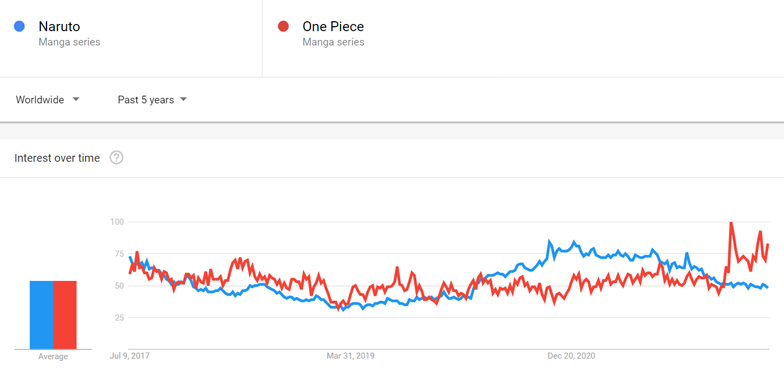
\includegraphics{quarto2_files/mediabag/naruto-vs-one-piece-.png}

}

\caption{Viewership Over Time}

\end{figure}

\hypertarget{episode-to-episode-changes-in-viewership}{%
\subsection{Episode-to-Episode Changes in
Viewership}\label{episode-to-episode-changes-in-viewership}}

\begin{figure}

{\centering 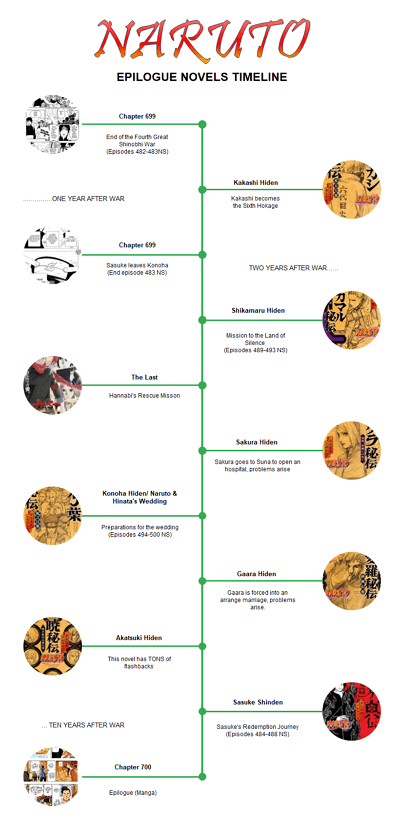
\includegraphics{quarto2_files/mediabag/naruto-novel-timelin.png}

}

\caption{Episode-to-Episode Changes}

\end{figure}

\hypertarget{observations-and-changes}{%
\subsection{Observations and Changes}\label{observations-and-changes}}

The viewership of \emph{Naruto} experienced notable fluctuations during
its broadcast. The transition from the initial \emph{Naruto} series to
\emph{Naruto: Shippuden} marked a significant turning point, with an
increase in viewership attributed to character growth and evolving
storylines.

Throughout the series, there were instances of viewership decline,
particularly during filler arcs that deviated from the main plot.
Despite these fluctuations, \emph{Naruto: Shippuden} maintained a
dedicated following, highlighting its enduring appeal.

The show's success can be attributed to its well-developed characters,
engaging story arcs, and exploration of themes such as friendship and
personal growth. \emph{Naruto} remains a beloved series with a lasting
impact on global anime culture.

\hypertarget{series-overview}{%
\subsection{Series Overview}\label{series-overview}}

\begin{figure}

{\centering 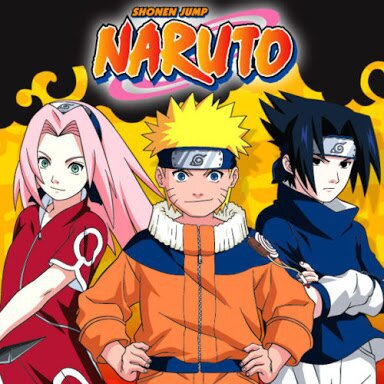
\includegraphics[width=2.08333in,height=1.5625in]{quarto2_files/mediabag/19726bbf6804a22d703d.jpg}

}

\caption{Naruto Shonen Jump}

\end{figure}

\begin{longtable}[]{@{}lll@{}}
\toprule\noalign{}
Season & Episodes & Originally Aired \\
\midrule\noalign{}
\endhead
\bottomrule\noalign{}
\endlastfoot
1 & 57 & October 3, 2002 - November 5, 2003 \\
2 & 43 & November 12, 2003 - September 8, 2004 \\
3 & 41 & September 15, 2004 - June 29, 2005 \\
4 & 42 & July 6, 2005 - May 3, 2006 \\
5 & 37 & May 10, 2006 - February 8, 2007 \\
\end{longtable}

\hypertarget{series-overview-1}{%
\subsection{Series Overview}\label{series-overview-1}}

\begin{figure}

{\centering \includegraphics{https://m.media-amazon.com/images/M/MV5BZGFiMWFhNDAtMzUyZS00NmQ2LTljNDYtMmZjNTc5MDUxMzViXkEyXkFqcGdeQXVyNjAwNDUxODI@._V1_.jpg}

}

\caption{Naruto Shipuden}

\end{figure}

\begin{longtable}[]{@{}llll@{}}
\toprule\noalign{}
Season & Episodes & First Aired & Last Aired \\
\midrule\noalign{}
\endhead
\bottomrule\noalign{}
\endlastfoot
1 & 32 & February 15, 2007 & October 25, 2007 \\
2 & 21 & November 8, 2007 & April 3, 2008 \\
3 & 18 & April 3, 2008 & August 14, 2008 \\
4 & 17 & August 21, 2008 & December 11, 2008 \\
5 & 24 & December 18, 2008 & June 4, 2009 \\
6 & 31 & June 11, 2009 & January 14, 2010 \\
7 & 8 & January 21, 2010 & March 11, 2010 \\
8 & 24 & March 25, 2010 & August 26, 2010 \\
9 & 21 & September 2, 2010 & January 27, 2011 \\
10 & 25 & February 10, 2011 & July 28, 2011 \\
11 & 21 & July 28, 2011 & December 28, 2011 \\
12 & 33 & January 5, 2012 & August 16, 2012 \\
13 & 20 & August 23, 2012 & January 10, 2013 \\
14 & 25 & January 17, 2013 & July 4, 2013 \\
15 & 28 & July 18, 2013 & January 30, 2014 \\
16 & 13 & February 6, 2014 & May 8, 2014 \\
17 & 11 & May 15, 2014 & August 14, 2014 \\
18 & 21 & August 21, 2014 & December 25, 2014 \\
19 & 20 & January 8, 2015 & May 21, 2015 \\
20 & 45 & May 28, 2015 & April 28, 2016 \\
21 & 21 & May 5, 2016 & October 13, 2016 \\
22 & 21 & October 20, 2016 & March 23, 2017 \\
\end{longtable}



\end{document}
